\documentclass{article}

\usepackage{amssymb}
\usepackage{amsmath}
\usepackage{graphicx}
\usepackage{authblk}

\title{L-Systems in Haskell}
\author[1]{Lucas Ferreira}
\author[1]{Sumukh Atreya}
\affil[1]{Department of Computer Science}
\affil[1]{University of California, Santa Cruz}

\date{\today}

\begin{document}
\maketitle

\abstract{
\noindent
This paper presents a technical report on the implementation of Lindenmayer Systems (or L-Systems)
using Haskell, a functional programming language. It is present as part of the requirements of
the \textit{CMPS203 - Programming Languages} course at \textit{University of California, Santa Cruz}.
One of the main motivations of this project is to develop experience in designing and
implementing good Haskell programs via real-world applications. L-Systems were selected
because of their recursive structure  and because they are very important in
the field of Procedural Content Generation, especially for the generation of tress and
forests.
}

\section{Introduction}

% Introduce the problem
Video games complexity has increased over the years, consequently the amount of content
(such as characters, maps, cities, etc) present in these games has also increased.
One of the main reasons for the increase in complexity of modern games is that the
virtual worlds contained on them are becoming more realistic. A common problem
when creating this worlds consists in designing forests, because of their organic
characteristics. Without the help of a computer, the designer would have to handcraft
every visible tree, in order to create a realistic scene.

% Introduce PCG
The time and effort spent producing these assets have motivated game developers to design
algorithms capable of generating content automatically. This approach is called Procedural
Content Generation (PCG) and it is often used in order to speed up the production
of content. In this case, developers have the opportunity to interact with PCG methods,
whose content created may be used as inspiration or starting point. These PCG methods must
care more about the novelty and diversity than quality or playability, since the developers
have the possibility to reject or edit any non-desired generated results. Several PCG
methods have been developed to support the generation of entire forests and one of
them is known as Lindenmayer Systems (or L-Systems).

% Introduce the solution
L-systems are generative grammars that define fractal patterns, which are useful to
the generation of content in video games and virtual worlds. It was originally defined
to describe the behavior of plant cells and to model the growth processes of plant development [0].
Later, it started being used for PCG in games [1], since this task has become increasingly demanding.
This paper presents a Haskell implementation of L-Systems, in partial fulfillment of the requirements for
the \textit{CMPS203 - Programming Languages} course of the \textit{University of California, Santa Cruz}.
The main motivation for using L-System to study Haskell is its recursive nature, which
is also how haskell process several data structures. Thus, this application
supports understanding how to design and implement good Haskell code.

This document is structured as follows: Section \ref{lsystems} defines L-Systems and
how they are used to produce fractal patterns. Section \ref{implementation} describes
the overall structure of the solution and the details of the Haskell implementation.
Section \ref{results} shows some examples of grammars and the outputs
generated by the implemented system. Finally, Section \label{conclusion} presents
a conclusion for this work.

\section{L-Systems}
\label{lsystems}

L-Systems are formal grammars and they are used to produce intricate and complex patterns
that are self similar across many scales. The L-System grammar consists of four components:

\begin{enumerate}
\item A set of variables that can be replaced using a set of production rules.
\item Constants, which are symbols that are not replaced.
\item The axiom, which is a string composed of variables and constants. It is the initial state of the system.
\item Production rules, which define the way that variables can be replaced by other variables and constants.
The production consists of a predecessor string and a successor string, which is obtained by applying the rules
 to the predecessor string.
\end{enumerate}

When the productions are applied to the axiom, they produce more strings. The rules can then be applied
to each of those strings to produce even more strings, and so on. For example, lets consider the system presented
in Table \ref{example1}, where the axiom is the string with three symbols ``peg'' and the set of production
rules is composed by only one element ``e=eie''.

\begin{table}[!h]
\centering
\begin{tabular}{|l|l|}
\hline
Axiom: & peg     \\ \hline
Rules: & e = eie \\ \hline
\end{tabular}
\label{example1}
\caption{An example of simple recursive L-System}
\end{table}

The single ``e'' symbol in the axiom is replaced with ``eie'' creating the string ``peieg''.
Since the rule in this L-system is recursive, the first generation string has two new ``e''
symbols, each of which get replaced with  ``eie'' in the second generation. This process goes
on until the desired amount of generations is reached. Table 2 shows the result of applying
the production tules for 3 generations on the system presented in Table \ref{example2}.

\begin{table}[]
\centering
\begin{tabular}{|l|l|}
\hline
Generation 1: & peieg             \\ \hline
Generation 2: & peieieieg         \\ \hline
Generation 3: & peieieieieieieieg \\ \hline
\end{tabular}
\label{example2}
\caption{The first three generations of strings produced by the L-System}
\end{table}

In order to use this system for generating plants and other visual artifacts, one
has to interpret them visually. A common way of doing that consists in using
the generated strings to control turtle graphics. Thus, constants are
used to move and turn a drawing robot, similar to the Logo programming language.
For instance, let's consider the grammar described in Table \ref{example3}.

\begin{table}[!h]
\centering
\begin{tabular}{|l|p{25mm}|}
\hline
Axiom: & FX        \\ \hline
Rules: & X = X+YF+ \newline Y = -FX-Y \\ \hline
\end{tabular}
\label{example3}
% \caption{An example of simple recursive L-System}
\end{table}

If the robot interprets F to mean ``move forward drawing one unit'' and - and + to
mean ``turn right 90 degrees'' and ``turn left 90 degrees'', respectively, then the robot will
draw what is illustrated in Figure \ref{fig:example} from the string generated
with 10 generations.

\begin{figure}[!h]
\centering
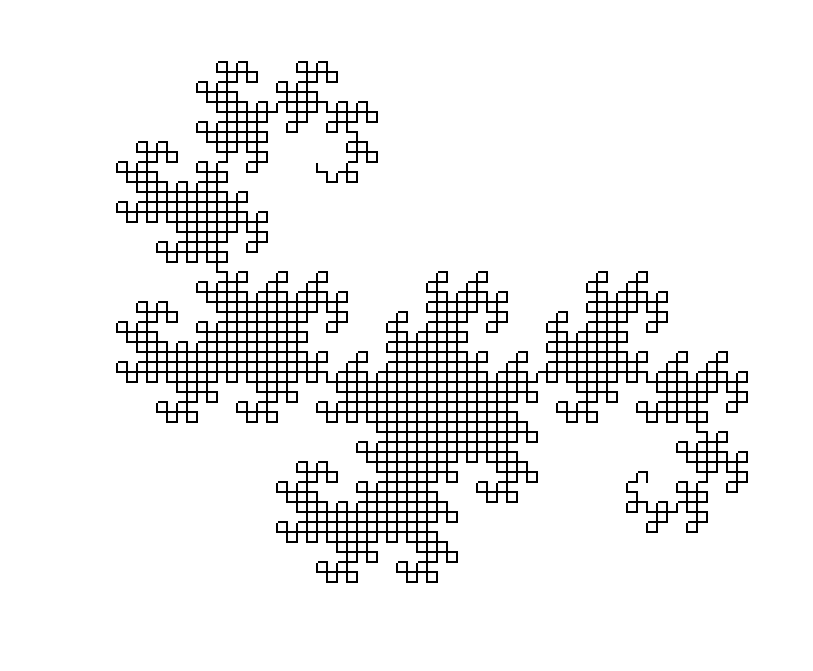
\includegraphics[width=0.48 \textwidth]{Images/result4.png}
\vskip -6pt
\label{fig:example}
\end{figure}

\section{Haskell Implementation}
\label{implementation}

The Haskell implementation presented in this paper uses the turtle graphics
structure defined in Section \ref{lsystems}. Grammars are defined in text files,
which are parsed into L-Systems. After, these systems are rendered using the \textit{Glos}
package, which is used to draw simple vector graphics on a window.

% In this section, we present the outline and provide a description of the implementation of the L-System in Haskell.
% In addition, we provide an overview of the major issues and difficulties encountered in the implementation of the system.

\begin{enumerate}
\item Parsing the input: The L-system takes as input the axioms, rules, the angle and the number of iterations. The first segment of the code parses the given input.
\item Parsing the L-Systems grammar: This part of the code takes as input a list of strings (containing the input) and returns an L-system.
\item Implementing the L-System: Here, the implementation of the L-system is carried out.
\item Rendering function:

\end{enumerate}

\section{Results}
\label{results}

\begin{figure}[!h]
\centering
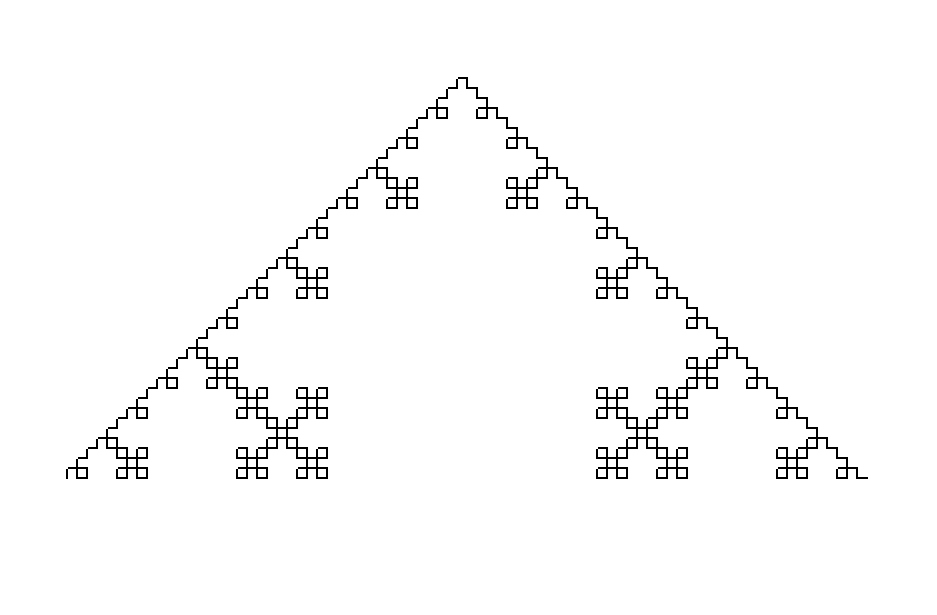
\includegraphics[width=0.48 \textwidth]{Images/result1.png}
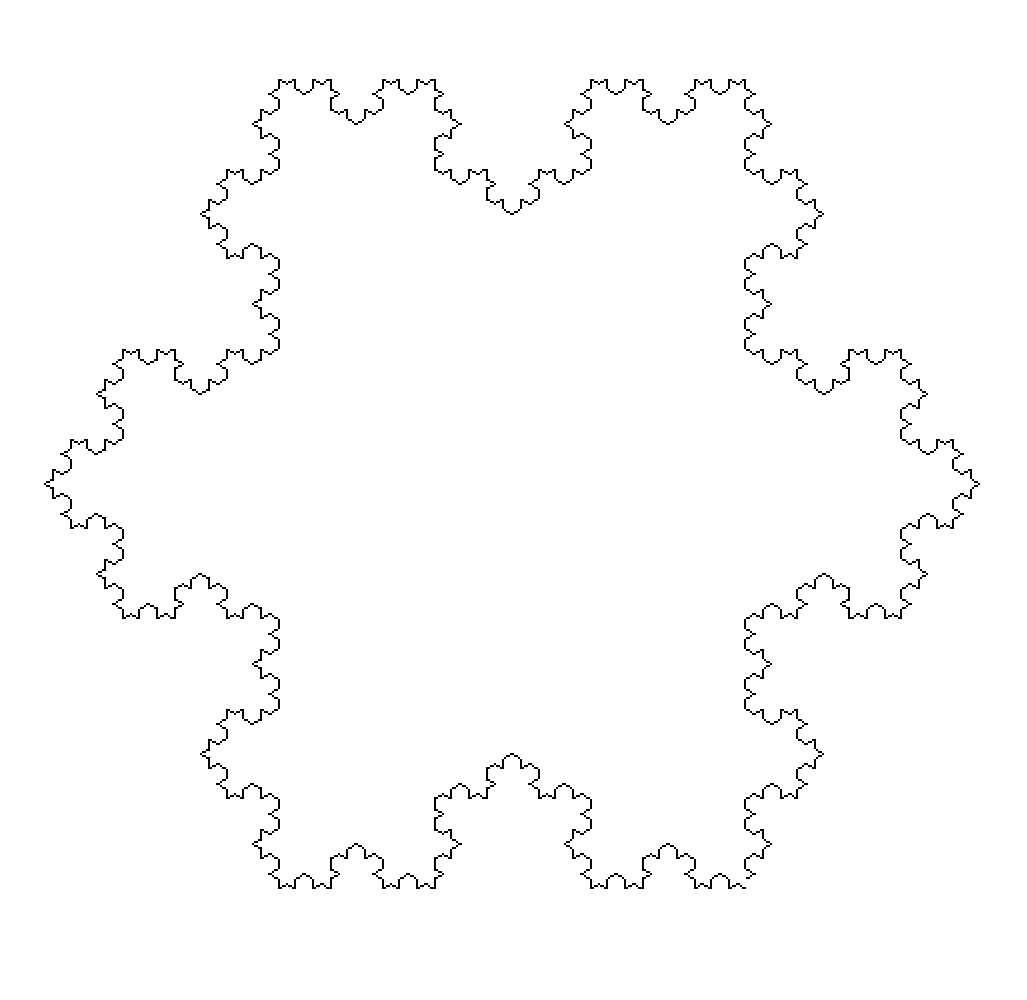
\includegraphics[width=0.48 \textwidth]{Images/result2.png}
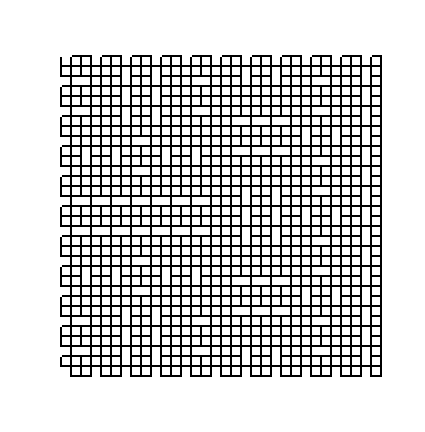
\includegraphics[width=0.48 \textwidth]{Images/result3.png}
\vskip -6pt
\label{fig:example_level}
\end{figure}

\section{Conclusion}
\label{conclusion}

\section{Appendix}

\end{document}
